\subsection{cudaMemcpy}
In comparison to d2h and h2d pinned and pageable memory transfer rates reported last week,
the device-to-device global memory access using cudaMemcpy outperforms at all data sizes.
The outperformance grows stronger towards larger data sizes where we reach transfer speeds
of up to 263 GB/s. This is because also on the device overhead dominates at small datasizes.
We are only able to get close to peak bandwidth once we reach larger data sizes approaching 1GB.
The d2d performance vastly outperforms the approximately 10 GB/s we get d2h or h2d over PCIe.


\begin{figure}
    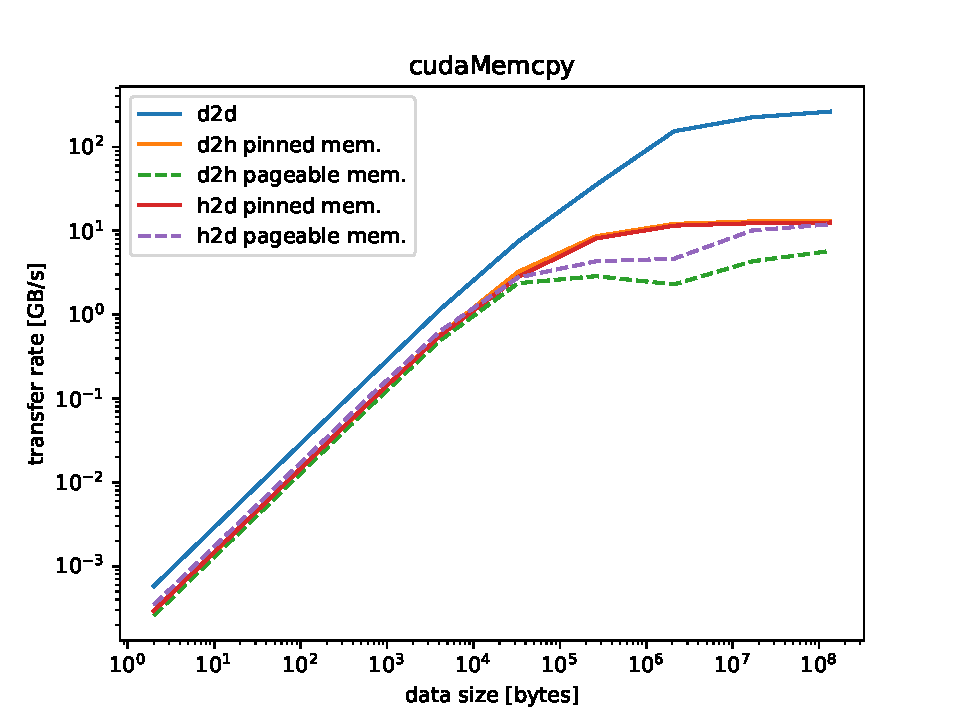
\includegraphics[scale=0.7]{cudaMemcpy.pdf}
    \caption{exercise 2.1, D2H/H2D pegeable, pinned and D2D}
    \label{fig:2.1}
\end{figure}
